\documentclass[12pt,a4paper,oneside]{article}

\usepackage[utf8]{inputenc}
\usepackage[portuguese]{babel}
\usepackage[T1]{fontenc}
\usepackage{amsmath}
\usepackage{amsfonts}
\usepackage{amssymb}
\usepackage{graphicx}
\usepackage{xcolor}
\usepackage{multicol}
% Definindo novas cores
\definecolor{verde}{rgb}{0.25,0.5,0.35}

\author{\\Universidade Federal de Jataí (UFJ)\\Bacharelado em Ciência da Computação \\Lógica para Ciência da Computação \\Esdras Lins Bispo Jr.}

\date{03 de abril de 2019}

\title{\sc \huge Mini-Teste 1}

\begin{document}

\maketitle

{\bf ORIENTAÇÕES PARA A RESOLUÇÃO}

\small
 
\begin{itemize}
	\item A avaliação é individual, sem consulta;
	\item A pontuação máxima desta avaliação é 10,0 (dez) pontos, sendo uma das 06 (seis) componentes que formarão a média final da disciplina: quatro mini-testes (MT), uma prova final (PF), exercícios em formato de {\it Quizzes} (QZ) e questões conceituais (QC) aplicadas em sala de aula pelo método de Instrução pelos Colegas;
	\item A média final ($MF$) será calculada assim como se segue
	\begin{eqnarray}
		MF & = & MIN(10, S) \nonumber \\
		S & = & [(\sum_{i=1}^{4} max(MT_i, SMT_i ) + PF].0,2  + QC + QZ\nonumber
	\end{eqnarray}
	em que 
	\begin{itemize}
		\item $S$ é o somatório da pontuação de todas as avaliações, e
		\item $SMT_i$ é a substitutiva do mini-teste $i$.
	\end{itemize}
	\item O conteúdo exigido desta avaliação compreende o seguinte ponto apresentado no Plano de Ensino da disciplina: (1) Lógica Proposicional.
\end{itemize}

\begin{center}
	\fbox{\large Nome: \hspace{10cm}}
\end{center}

\newpage

\begin{enumerate}
	
	\section*{Primeiro Teste}
	
	\item (5,0 pt) Sejam as proposições $p$: ``O sistema tem uma tela de login'', e $q$: ``O usuário está autenticado''. Traduza as duas proposições abaixo:
	\begin{enumerate}
		\item (2,5 pt) {\bf [para a linguagem natural]} \\$\sim q \rightarrow \sim p$
		\vspace*{0.3cm}
		
		\item (2,5 pt) {\bf [para a linguagem simbólica]} \\Não é verdade que o sistema tem uma tela de login e o usuário não está autenticado.
	\end{enumerate}
	
	
	\item (5,0 pt) Informe os todos valores lógicos das duas regiões 3x3 (R1 e R2) que estão faltando na tabela-verdade abaixo.
		\begin{center}
			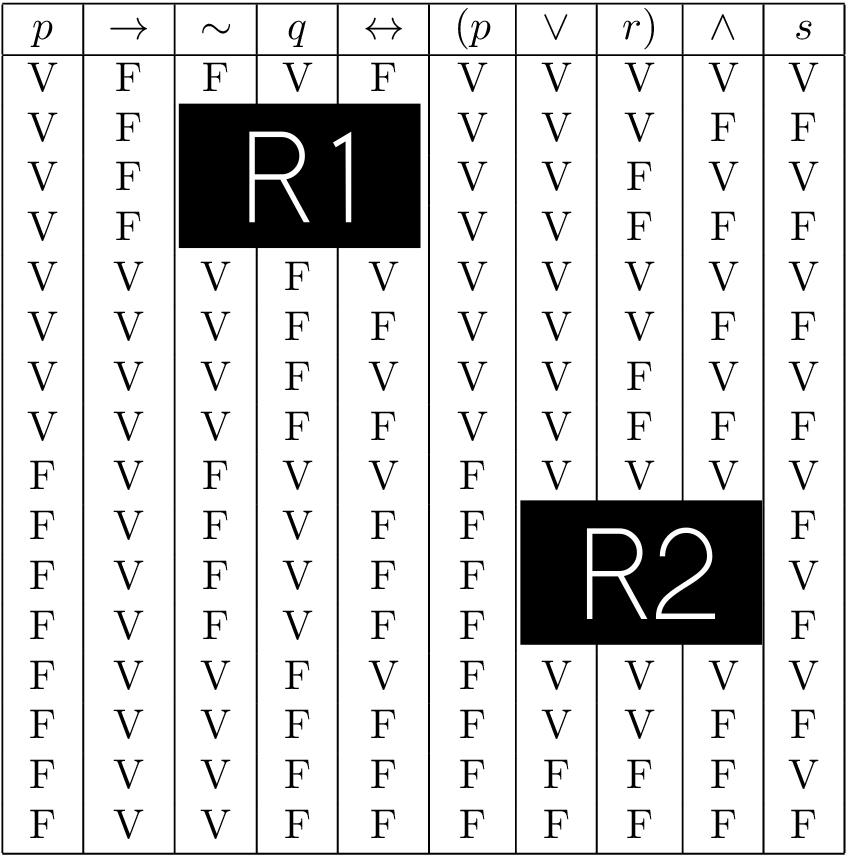
\includegraphics[width=\textwidth]{images/tv-regiao.png}
		\end{center}
	
%	\begin{tabular}{|c|c|c|c|c|c|c|c|c|c|}
%		\hline
%		$p$ & $\rightarrow$ & $\sim$ & $q$ & $\leftrightarrow$ & $(p$ & $\vee$ & $r)$ & $\wedge$ & $s$  \\
%		\hline
%		V & F & F & V & F & V & V & V & V & V \\
%		V & F & F & V & V & V & V & V & F & F \\
%		V & F & F & V & F & V & V & F & V & V \\
%		V & F & F & V & V & V & V & F & F & F \\
%		V & V & V & F & V & V & V & V & V & V \\
%		V & V & V & F & F & V & V & V & F & F \\
%		V & V & V & F & V & V & V & F & V & V \\
%		V & V & V & F & F & V & V & F & F & F \\
%		F & V & F & V & V & F & V & V & V & V \\
%		F & V & F & V & F & F & V & V & F & F \\
%		F & V & F & V & F & F & F & F & F & V \\
%		F & V & F & V & F & F & F & F & F & F \\
%		F & V & V & F & V & F & V & V & V & V \\
%		F & V & V & F & F & F & V & V & F & F \\
%		F & V & V & F & F & F & F & F & F & V \\
%		F & V & V & F & F & F & F & F & F & F \\
%		\hline
%	\end{tabular}

\end{enumerate}

\end{document}